% ═══════════════════════════════════════════════════════════════════
% Figure captions for:
% "Rambling and Trembling as Distinct Components of the
%  Closed Postural Control Circuit"
% ═══════════════════════════════════════════════════════════════════

\begin{figure*}[!htbp]
    \centering
    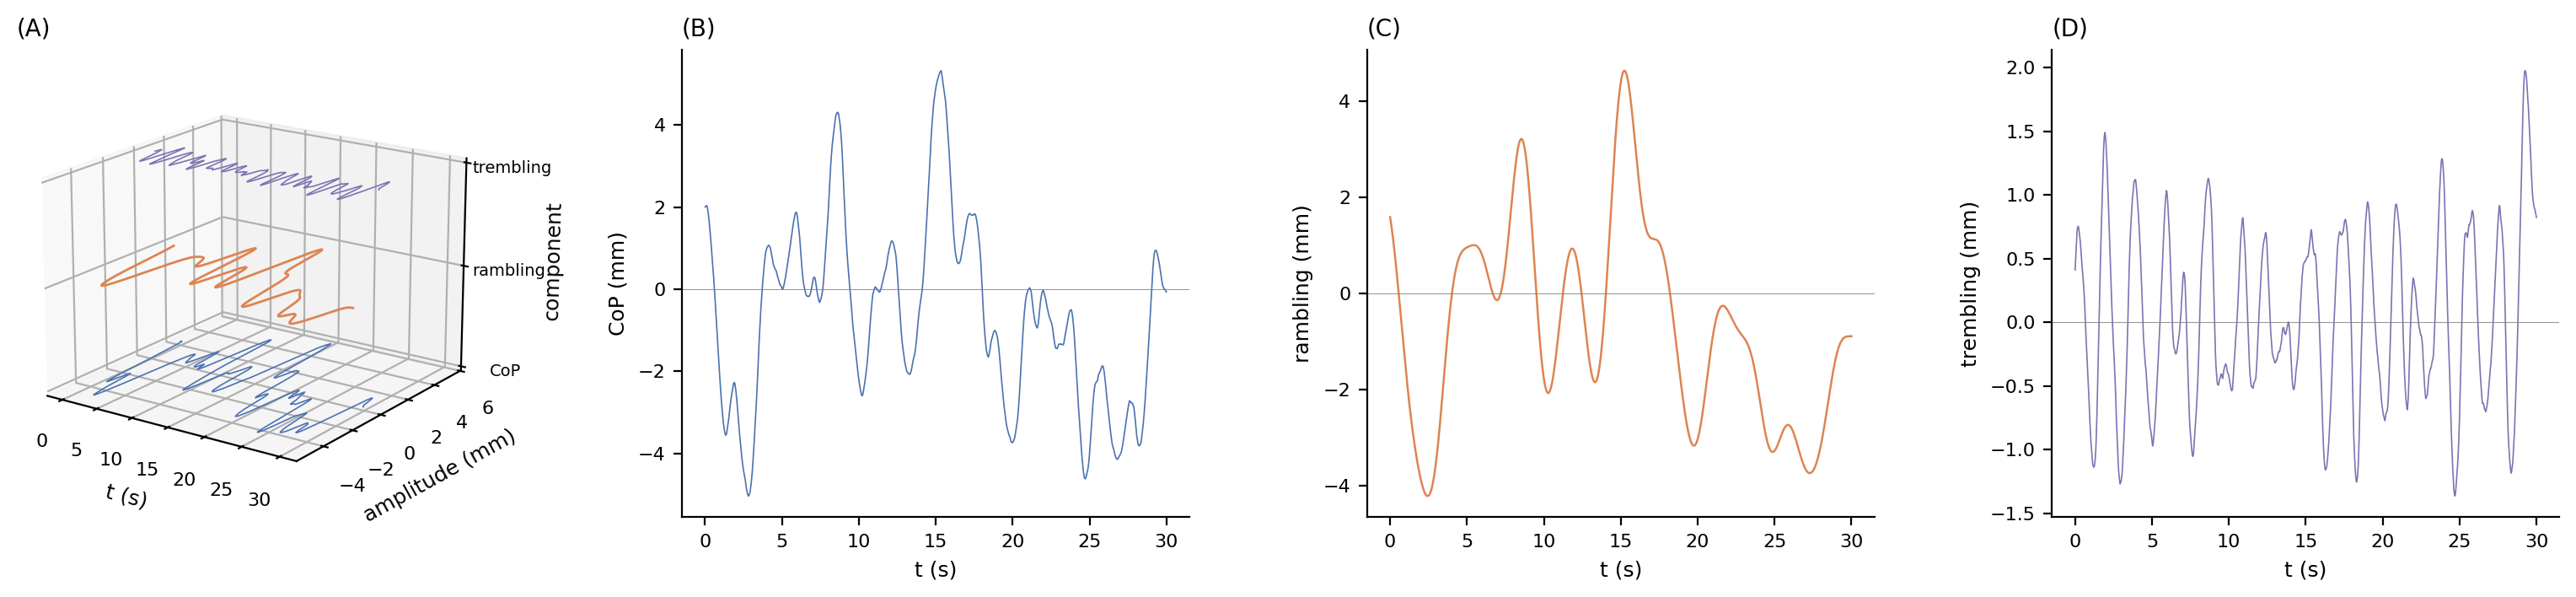
\includegraphics[width=\textwidth]{figures/panel1_decomposition.png}
    \caption{\textbf{IEP Decomposition of Center-of-Pressure into Rambling and Trembling.}
    (\textbf{A})~Three-dimensional stack plot of the center-of-pressure trajectory and its two decomposition components. Three traces are offset along the vertical axis at $z = 0$ (CoP, blue), $z = 10$ (rambling, orange), and $z = 20$ (trembling, purple). The original CoP trace contains the full $30$\,s of simulated quiet standing at $200$\,Hz. The two components are extracted by fourth-order Butterworth low-pass filtering at $0.4$\,Hz, with rambling being the low-pass portion and trembling the residual.
    (\textbf{B})~Original CoP time series, showing continuous bounded oscillation with root-mean-square displacement $2.24$\,mm and peak-to-peak range $\sim 8$\,mm. The subject never reaches a static position; the oscillation is the signature of the closed postural circuit maintaining upright posture without external ground.
    (\textbf{C})~Rambling component ($\mathrm{CoP}_{\mathrm{Ra}}$). The slow drift captures the slowly varying reference configuration of the postural circuit, reflecting supraspinal integration on time scales of $1$--$5$\,s. RMS amplitude $\approx 1.8$\,mm, dominated by content below $0.4$\,Hz.
    (\textbf{D})~Trembling component ($\mathrm{CoP}_{\mathrm{Tr}}$). High-frequency deviations about the rambling trajectory, reflecting the bounded oscillation of spinal stretch reflex loops about the momentary reference. RMS amplitude $\approx 0.7$\,mm, with power concentrated in the $0.4$--$3$\,Hz band. The two components sum exactly to the original CoP, with reconstruction error below numerical precision.}
    \label{fig:decomposition}
\end{figure*}


\begin{figure*}[!htbp]
    \centering
    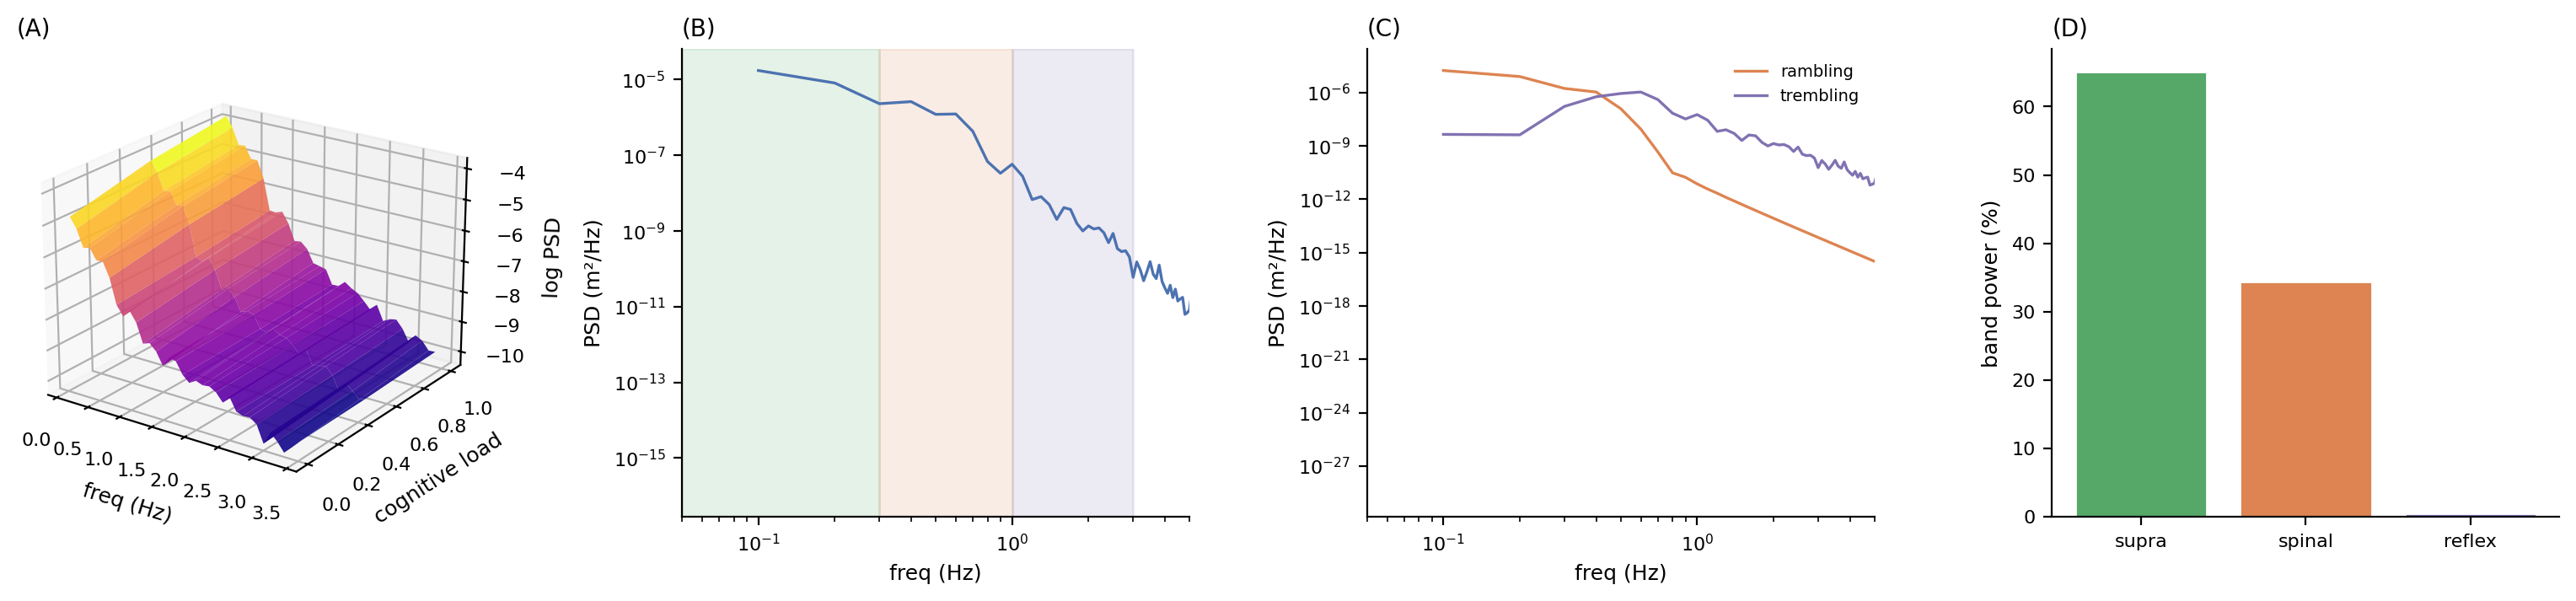
\includegraphics[width=\textwidth]{figures/panel2_spectral.png}
    \caption{\textbf{Spectral Structure of the Postural Circuit.}
    (\textbf{A})~Three-dimensional power spectral density surface over $(f, L_{\mathrm{cog}})$, where $f$ is frequency and $L_{\mathrm{cog}} \in \{0.0, 0.5, 1.0\}$ is the imposed cognitive load. Each sheet of the surface is a Welch periodogram (10\,s segments, Hann window) of $30$\,s of simulated CoP. Log power is plotted. The surface shows systematic elevation of low-frequency power with increasing cognitive load, corresponding to the preferential rambling-band effect.
    (\textbf{B})~Baseline CoP power spectrum on log--log axes. Three spectral bands are highlighted: supraspinal slow-drift ($0.05$--$0.3$\,Hz, green), spinal loop ($0.3$--$1$\,Hz, orange), and reflex band ($1$--$3$\,Hz, purple). The characteristic $1/f^{\alpha}$ decay across bands is consistent with coupled multi-level oscillator dynamics \citep{duarte2008,collins1993}.
    (\textbf{C})~Power spectra of rambling (orange) and trembling (purple) components extracted by IEP decomposition. Rambling power is concentrated below the $0.4$\,Hz decomposition cutoff; trembling power extends from $0.4$ to $\sim 3$\,Hz. The complementary spectral support confirms that the decomposition captures genuinely distinct frequency regimes rather than arbitrary filter-induced partitioning.
    (\textbf{D})~Band-power percentages in the full CoP spectrum. The supraspinal band contains $\sim 65\%$ of total power, the spinal band $\sim 34\%$, and the reflex band $\sim 1\%$. The distribution reflects the inverted-pendulum dynamics, in which low-frequency dynamics dominate the kinematic output while high-frequency content primarily appears in force and EMG signals.}
    \label{fig:spectral}
\end{figure*}


\begin{figure*}[!htbp]
    \centering
    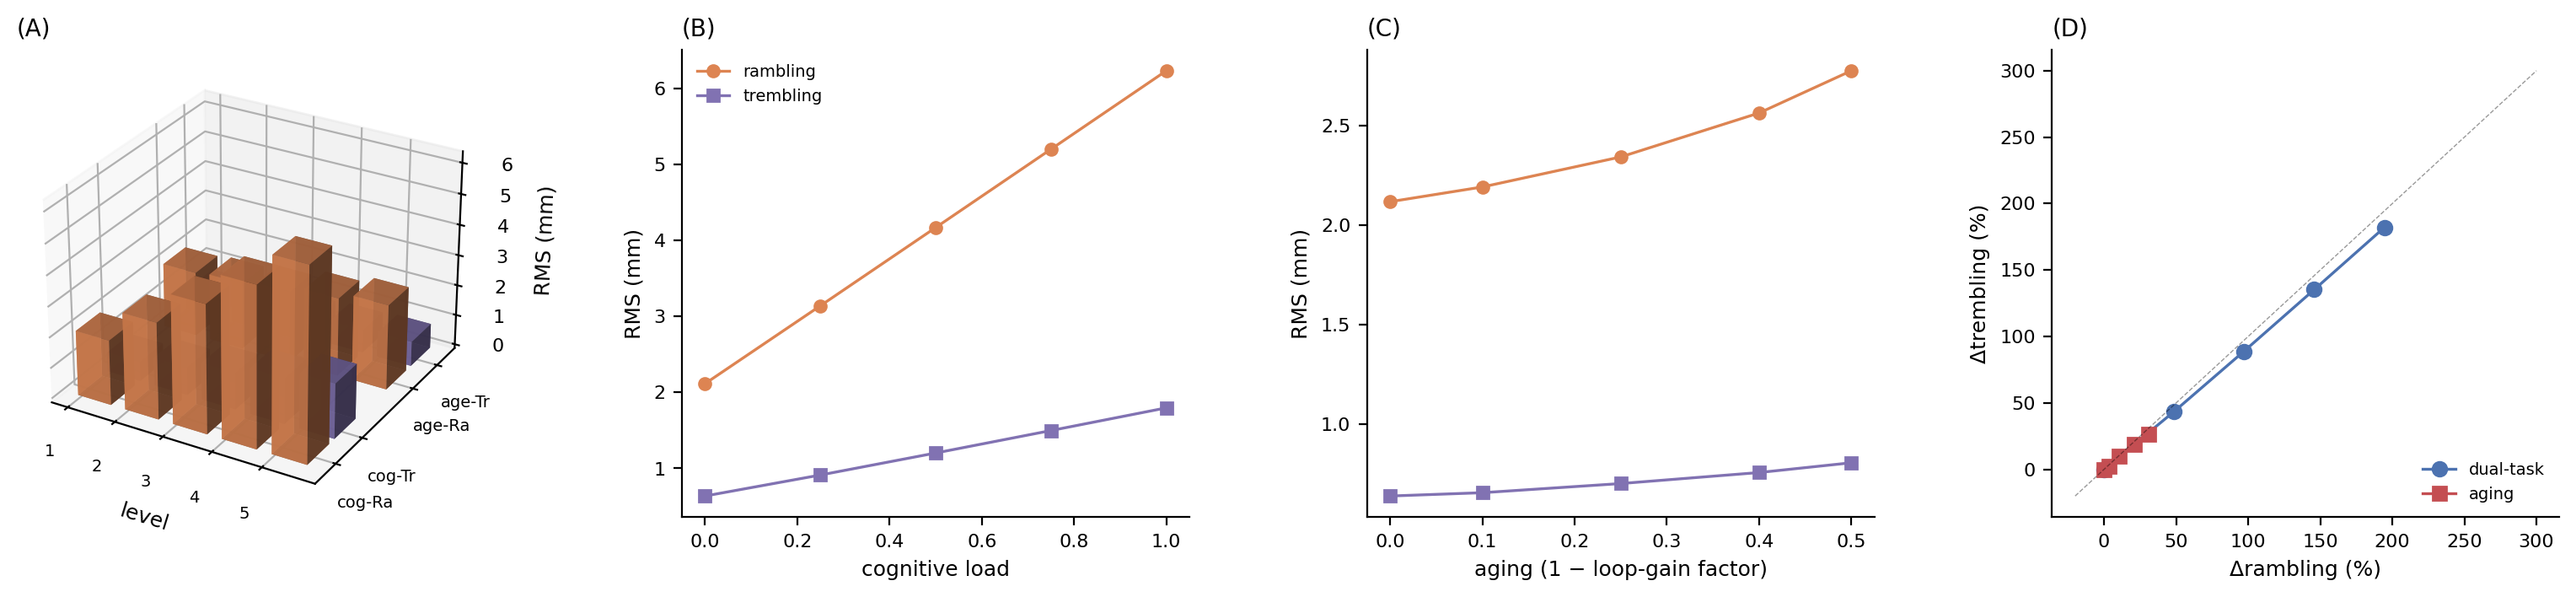
\includegraphics[width=\textwidth]{figures/panel3_dual_task_aging.png}
    \caption{\textbf{Dual-Task and Aging Effects on Rambling and Trembling.}
    (\textbf{A})~Three-dimensional bar chart of rambling (orange) and trembling (purple) amplitudes across five conditions for cognitive load and five for aging. Each bar is the mean of three seeds. The cognitive-load cluster (front) shows large growth in rambling with modest growth in trembling; the aging cluster (rear) shows opposite preferential growth in trembling with smaller rambling change.
    (\textbf{B})~Rambling (orange) and trembling (purple) RMS amplitudes versus cognitive load for levels $L_{\mathrm{cog}} \in \{0.0, 0.25, 0.5, 0.75, 1.0\}$. Rambling amplitude rises from $\sim 2.1$\,mm at baseline to $\sim 6.2$\,mm at maximum load (a $\sim 195\%$ increase). Trembling amplitude also rises (by $\sim 167\%$) but remains well below the rambling curve. The preferential effect on rambling is consistent with the empirical dual-task literature \citep{lajoie1993,pellecchia2003}.
    (\textbf{C})~Rambling and trembling versus aging severity (plotted as $1 - $loop-gain-factor, so increasing aging is toward the right). Rambling amplitude rises modestly from $\sim 2.1$\,mm to $\sim 2.7$\,mm ($32\%$ increase); trembling amplitude rises slightly more ($36\%$). The aging effect is smaller in absolute terms than the cognitive-load effect and affects the two components with more similar magnitudes, reflecting that age-related loop-gain reduction disrupts the whole circuit rather than selectively one level.
    (\textbf{D})~Scatter of $\Delta$trembling\,(\%) versus $\Delta$rambling\,(\%) for the cognitive-load (blue) and aging (red) trajectories. The dashed diagonal marks equal proportional change. Both trajectories lie approximately on or below the diagonal, indicating that in both perturbations rambling changes at least as much as trembling. The cognitive-load trajectory has larger overall excursion, matching the empirical observation that cognitive interference produces the strongest rambling effects.}
    \label{fig:dual_task_aging}
\end{figure*}


\begin{figure*}[!htbp]
    \centering
    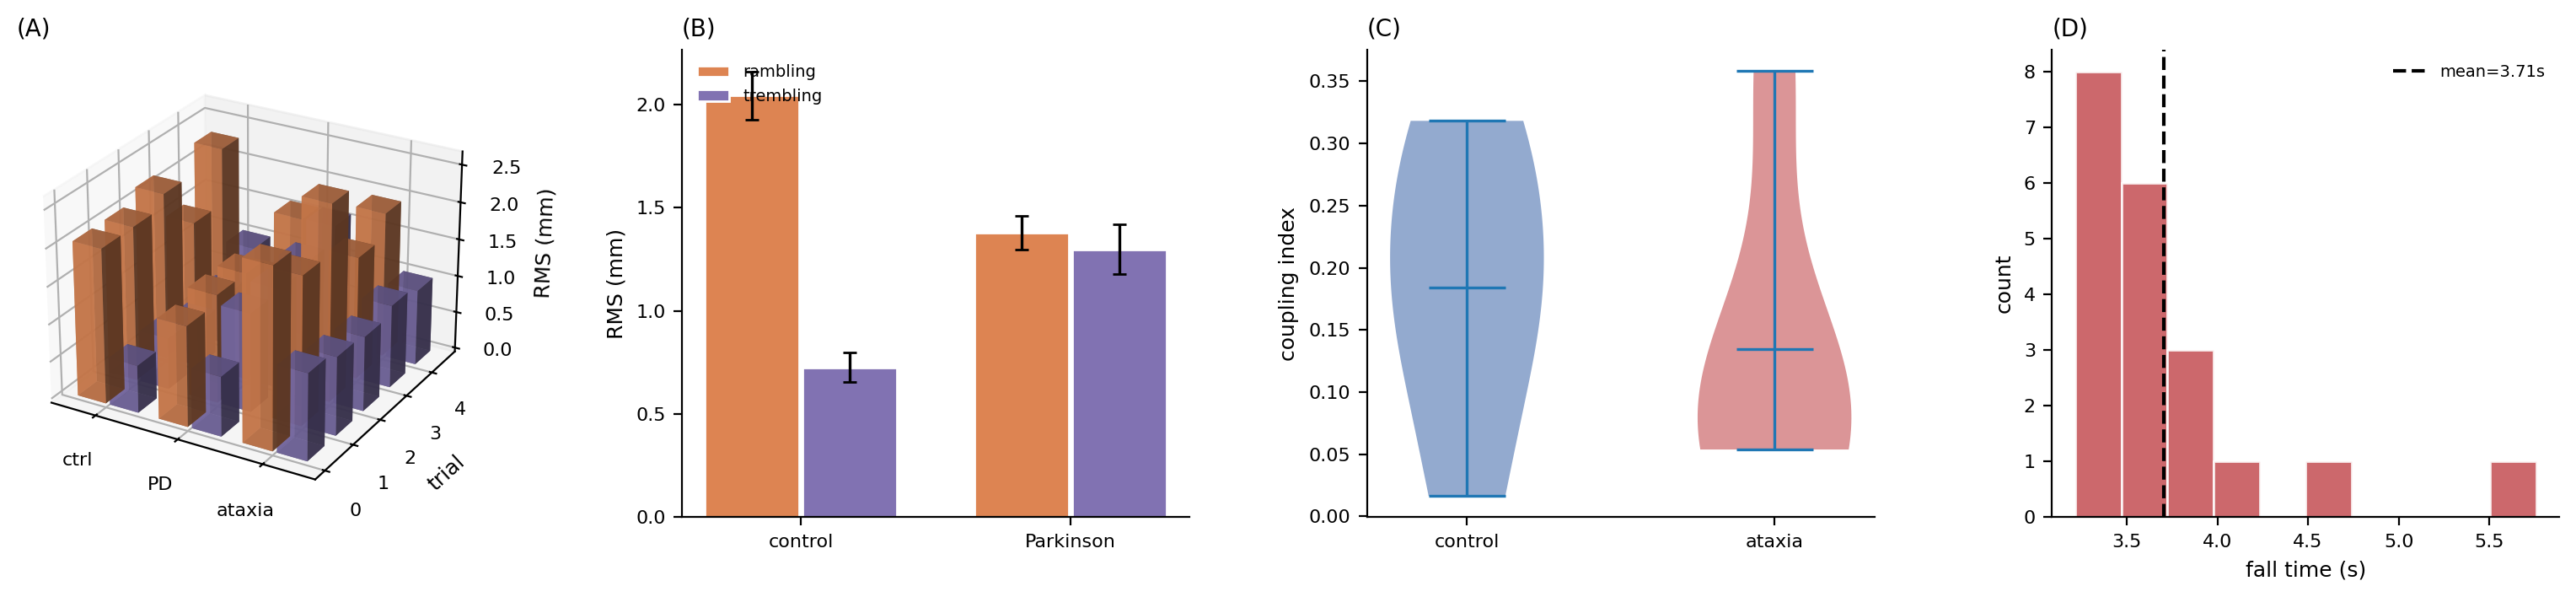
\includegraphics[width=\textwidth]{figures/panel4_pathology.png}
    \caption{\textbf{Pathology-Specific Signatures in Rambling--Trembling Structure.}
    (\textbf{A})~Three-dimensional clustered bar chart of rambling (orange) and trembling (purple) amplitudes across three conditions (control, Parkinson's disease [PD], cerebellar ataxia) and five seeds per condition. Control shows the largest rambling-to-trembling ratio; PD shows compressed rambling with elevated trembling; ataxia shows elevated variability in both components.
    (\textbf{B})~Mean rambling and trembling RMS for control and Parkinson's disease, with standard errors across five seeds. Controls: rambling $\approx 2.0$\,mm, trembling $\approx 0.7$\,mm. Parkinson's: rambling $\approx 1.4$\,mm ($-33\%$), trembling $\approx 1.3$\,mm ($+79\%$). The convergence of the two components is the characteristic Parkinsonian signature: reduced voluntary postural bias modulation with elevated spinal-loop oscillation from reduced damping.
    (\textbf{C})~Rambling--trembling coupling index ($C_{\mathrm{Ra,Tr}}$, magnitude of cross-correlation between rambling and trembling envelope) shown as violin plots for control (blue) and simulated cerebellar ataxia (red). Controls: median $\approx 0.18$, interquartile range extending to $0.32$. Ataxic: median $\approx 0.14$, with long tail toward $0.05$. The coupling drop reflects disrupted phase regulation between supraspinal and spinal components, the predicted signature of cerebellar timing-regulator loss.
    (\textbf{D})~Distribution of fall times for $20$ seeds of deafferented standing (proprioceptive return removed). All $20$ trials end in falls; fall times cluster around $3.7$\,s with a right tail extending to $5.7$\,s. The mean fall time (dashed line) is $3.71$\,s. The $100\%$ fall rate matches the clinical observation that deafferented patients collapse immediately on eye closure, confirming that the postural circuit cannot close without a proprioceptive return path.}
    \label{fig:pathology}
\end{figure*}


\begin{figure*}[!htbp]
    \centering
    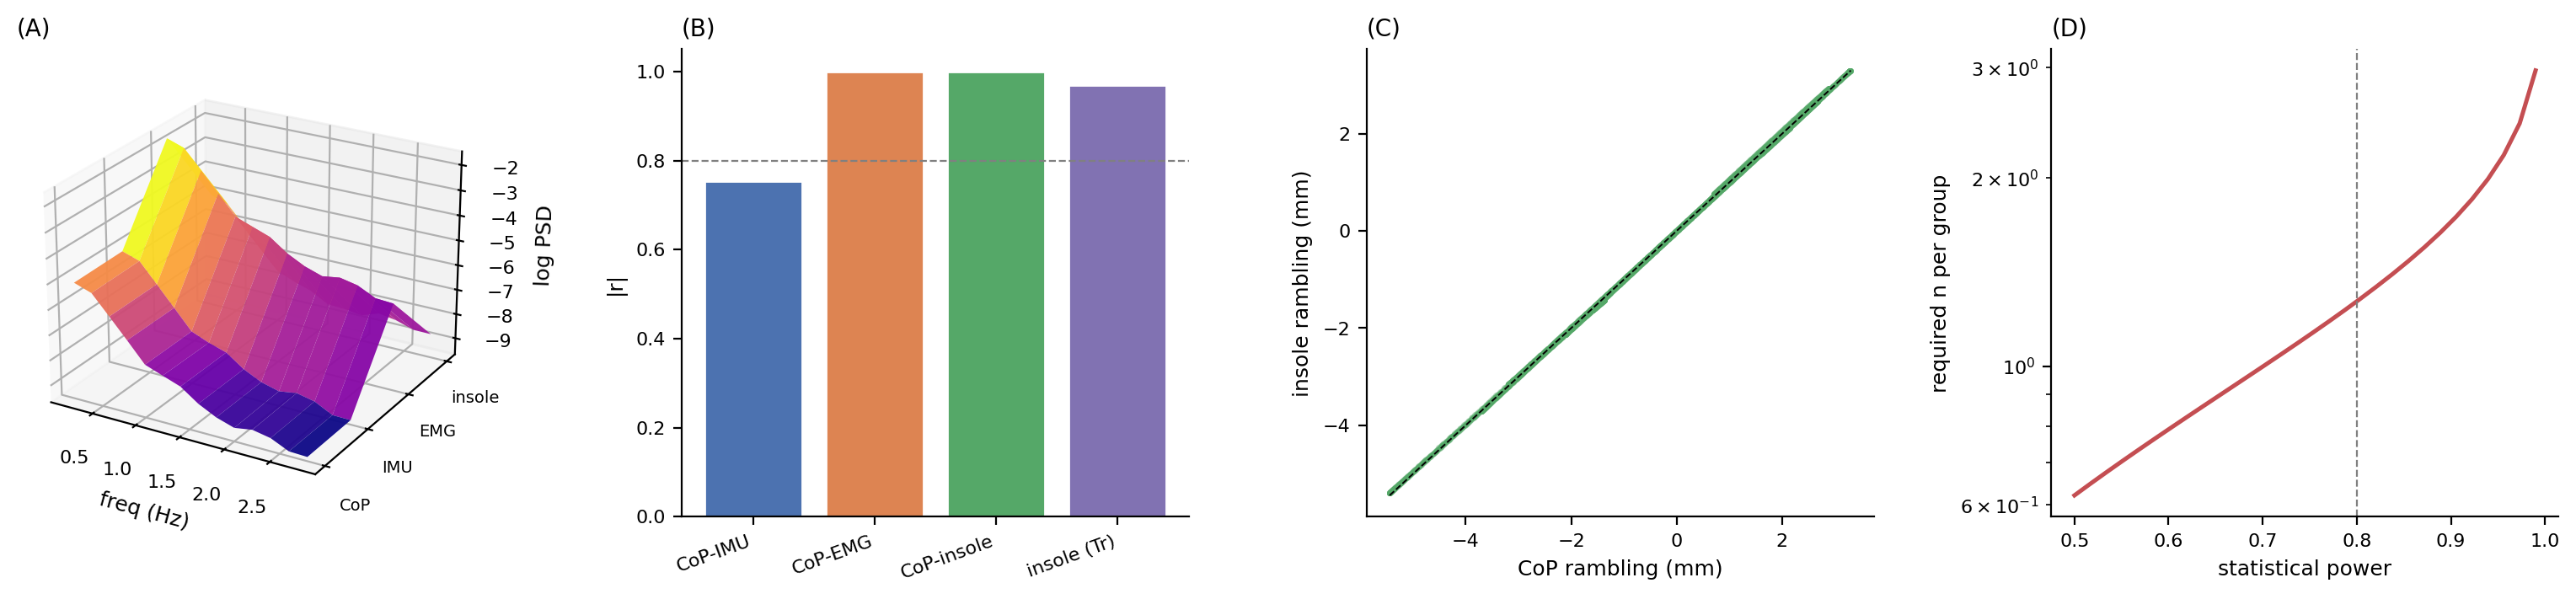
\includegraphics[width=\textwidth]{figures/panel5_multisensor.png}
    \caption{\textbf{Multi-Sensor Consistency and Statistical Power.}
    (\textbf{A})~Three-dimensional log-PSD surface over $(f, \mathrm{sensor})$ for four simulated sensor modalities applied to the same underlying postural dynamics: force-plate CoP, smartphone/smartwatch IMU (integrated from accelerometer), wrist-patch EMG envelope, and pressure-sensing insole. All four modalities show spectral support below $3$\,Hz with overlapping structure in the postural-loop band, demonstrating that different transduction principles capture consistent features of the underlying charge-circuit dynamics.
    (\textbf{B})~Cross-sensor absolute correlations of the rambling component after amplitude calibration to the CoP reference. CoP--IMU, CoP--EMG, CoP--insole, and insole-trembling all exceed the dashed threshold ($r = 0.8$), confirming that the decomposition is recoverable from each modality. The insole, with its direct pressure measurement, achieves near-perfect agreement with the force-plate CoP ($r > 0.99$).
    (\textbf{C})~Scatter plot of calibrated insole rambling versus force-plate CoP rambling. The diagonal (dashed) marks perfect agreement. The scatter clusters tightly around the identity line, demonstrating that consumer-grade pressure insoles can recover the rambling component of postural sway with precision sufficient for clinical applications.
    (\textbf{D})~Required sample size per group (log scale) as a function of statistical power for detecting the Parkinson's trembling elevation effect ($d = 3.17$). Vertical dashed line marks conventional $80\%$ power; required $n$ at this power is $\sim 1.3$ per group, reflecting the very large simulated effect size. At stringent $99\%$ power, required $n$ rises to $\sim 3$. The curve establishes feasibility of Parkinson's screening with small cohort sizes.}
    \label{fig:multisensor}
\end{figure*}
